\documentclass{article}
\usepackage{algorithm}
\usepackage{algpseudocode}
\usepackage{natbib}
\usepackage{graphicx}
\usepackage{amsmath}
\usepackage{hyperref}
\usepackage{caption}
\usepackage{multirow}
\usepackage{float}
\usepackage{booktabs,siunitx}
\sisetup{%
  output-decimal-marker={,},
}
\hypersetup{
colorlinks=false,
pdfborder={0 0 0},
}
\title{Systemic risk and financial connectedness: empirical evidence}
\bibliographystyle{apalike}
\author{Mateusz Dadej}
\date{\today}

\begin{document}

\maketitle

\subsection*{Introduction}

One of the main contributions of literature on financial networks is the property of financial system called robust-yet-fragile. The term was first coined by chief economist of Bank of England, Andrew Haldane (\citet{haldane}). He posits that financial connections can serve at the same time as shock-absorbers and shock-amplifiers to the financial sector. This makes the system robust, when the magnitude of shock is relatively small, but fragile, when the shock is large. 

A seminal paper by \citet{acemoglu}, provides a formal model, in which an extent of financial contagion exhibits a form of regime transition. When the shocks are small, the damages are dissipated through large number of financial institutions. On the other hand, when the shock is above some threshold, the properties of the system changes markedly. The damages are no longer dissipated, but amplified through the network. This makes the effect of connectedness on the system regime-dependent. Similar works that provide a theoretical mechanisms this property are \citet{callaway} and \citet{gai}

This research aims at providing empirical evidence for the regime-dependent effect of connectedness on financial stability. 

\subsection*{Research design}

The research design is a two step process. Using stock prices data of the biggest banks from eurozone and US, various statistical measures of system connectedness are estimated. The measures are calculated on a rolling basis, providing the time series of connectedness. 

In the second step, in order to assess the regime-dependent effect of connectedness on financial stability, the time series of connectedness is used as an explanatory variable in a Markov switching ARCH model.

\subsection*{Measures of financial connectedness}

Because of lack of transaction-level data among banks, the econometric literature provides several methods that aim at estimating a level of connectedness of financial sector. The measures are all estimated based on stock prices data, therefore providing a relatively high frequency variables. 

\

\textbf{1. Average correlation} 

\[\bar{\rho}(R) = \frac{\sum_{i \neq i}^{N} \sum_{j \neq j}^{N} \rho_{i,j}(R)}{N^2-N}\]

Where $\rho_{i,j}(R)$ is a correlation matrix of rate of returns, estimated with a Ledoit-Wolf estimator (\citet{ledoit}). This estimator is shown to have smaller estimation error than sample covariance when the number of observations is relatively small. This is the case for the research design, where the measures of financial connectedness are estimated on a rolling basis. The measure calculates the average correlation across the banks in the sample. The higher the average correlation, the more connected the system is.

\

\textbf{2. Covariance eigenvalue }

Given the sample covariance matrix of rates of returns $\Sigma$, the covariance eigenvalues $\lambda$ are obtained solving the below equation:

\[|\bf{A} - \lambda \bf{I}| = 0\]

The eigenvalues based measure of connectedness is then defined as:

\[\frac{\sum_{i}^{k} \lambda_i}{\sum_{i}^{N} \lambda_i}\]

This measure captures the proportion of variance of the system that is explained by the first $k$ eigenvalues, as in the principal component analysis. The higher the proportion, the more connected the system is.

\

\textbf{3. Granger causality network degree}

This measure is based on the Granger defined causality (\citet{granger}). In which a time-series variable $x_t$ "granger" cause variable $y_t$, when it contains enough information at time $t$ to predict value of $y_{t+1}$. 

Specifically, the granger causality is investigated with following regression:

\[r_{i,t+1} = \beta_0 + \beta_1 r_{m, t} + \beta_2 r_{j, t}\]

Where $r_{j, t}$ is a rate of return of bank $j$ at time $t$, which allegedly granger causes the rate of return of bank $i$. The regression also controls for the market rate of return $r_{m, t}$, which is a proxy for the market changes.

The banks $j$ and $i$ are said to be connected when the coefficient $\beta_2$ is statistically significant. 

Given the procedure above we can define an adjacency matrix $G$ describing the relationship between the banks:

\[G_{i,j} = \begin{cases}
    1  & \text{if } j \text{ granger cause } i \\
    0 & \text{otherwise}
  \end{cases} \forall i \neq j\]

Then the measure of granger connectedness is defined as:

\[\frac{\sum_{i \neq j}^{N} \sum_{j \neq i}^{N} G_{i,j}}{ N \times (N-1)}\]

The last two of the above connectedness measures are as described in \citet{billio}.

\subsection*{Modeling the regime-dependent effect of connectedness}

As the theory suggests, the effect of connectedness on financial stability is regime-dependent. In order to capture this property, a Markov switching ARCH model is used to describe the time-varying volatility of banking sector. The proxy of the banking sector being the appropriate banking index (eurozone or US banking sector index, maintained by S\&P or STOXXX).

The mean specification of the model controls for the first order autocorrelation of the broad market rate of returns (S\&P 500 or STOXX600) and an autoregressive component:

\[\mu_{i,t} = \beta_0 + \beta_1 r_{b,t-1} + \beta_1 r_{m,t-1} + \underbrace{\sigma_t z_t}_{=\epsilon_t}\]

Where $r_{b,t}$ is the rate of return of the banking sector index and $r_{m,t}$ is the rate of return of the broad market index. The Markov-switching ARCH specification is then:

\[\sqrt{\sigma^2_t} = \alpha_{0,s} + \alpha_{1,s} \kappa_{t-1} + \sum_{i=1}^{p} \alpha_{i+1} \sqrt{\epsilon^2_{t-i}}\]

With $z_t \sim \text{i.i.d.} \mathcal{N}(0, \eta_s)$. The $p$ is the number of lags of the ARCH effect (The models are estimated with $p = 4$). The model parameters indexed with $s$ are regime-dependent. Differentiating the effect of connectedness on the banking volatility for different market conditions. The regime is described by the Markov process $s_t$ with transition probabilities $\pi_{ij}$:

\begin{equation*}
  P(S_t = i | S_{t-1} = j) = \begin{bmatrix}
    \pi_1 & 1 - \pi_2\\
      1 - \pi_1 & \pi_2
      \end{bmatrix}
\end{equation*}

Unlike in usual specification of ARCH class models, the $\alpha$ parameters are unconstrained. Since we are interested in the effect of connectedness, instead of predicting the volatility, the parameters should be free to take any value.

A well documented phenomena is the increase of the correlation across assets during the financial distress. This is mostly because of the fly to safety effect and search for liquidity. In order to avoid this endogeneity, the connectedness measures are lagged by one period, thus providing a causal effect on the volatility of banking sector.

The model is estimated first by fitting the linear model with mean specification and then the Markov switching model to the root-squared residuals and their lags. 

\subsection*{Data and preprocessing}

The data used in the research is the daily stock prices of the banks from two regions - US and Europe. The banks from the sample needs to take part in the EBA stress tests (\citet{eba}) or Fed stress tests (\citet{fed}) and be publicly traded. The total amount of the banks in the sample is 41 for EU and 30 for US. S\&P and STOXX600 are used for the broad market index and their relative industry specific indices. The data is from 2000 to 2023.

For comparability, the connectedness measures are standardized to have mean 0 and standard deviation 1. The final time series for EU are presented in figure 1. The absolute returns of stocks and indices are multiplied by 100. The eigenvalue based measure is calculated based on a single highest eigenvalue. 

\begin{figure}[H]
  \caption{Time series of connectedness measures for a rolling window of 63 trading days (quarter)}
  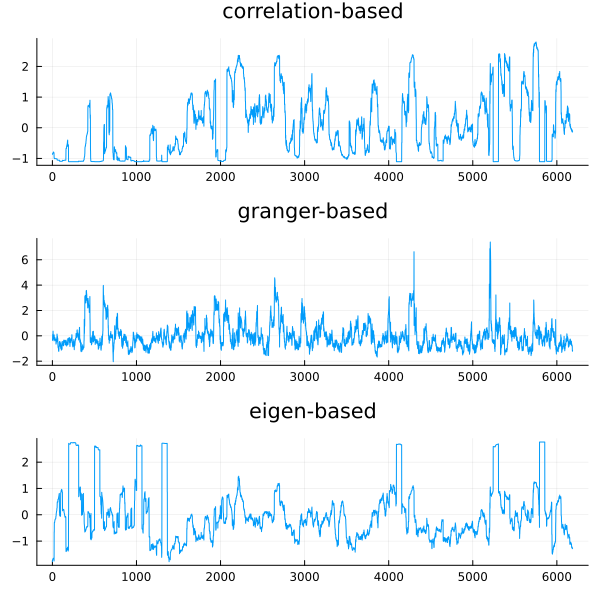
\includegraphics[scale=0.5]{connectmeasures.png}
  \centering
\end{figure}

\

\subsection*{Results}

The results are presented below. Parameters of the mean specifications ($\beta$) and parameters of ARCH effects ($\alpha_{2,\cdots,p}$) are omitted for the sake of brevity (almost always positive and statistically significant). The $\pi_{i,i}$ are diagonal elements of the transition matrix.

The model distinguished two regimes. The first one can be briefly described as low-volatility regime (with lower $\alpha_0$ and $\eta$), while the second one as high-volatility regime. Unsurprisingly, the transition probabilities suggests that the former one is less prevalent. 

The models provide partial evidence in favor of the robust-yet-fragile narrative. During low-shock regime, the connectedness plays a negligible role. Although, the effect is often statistically significant and positive, the magnitude is always economically irrelevant. Ranging from $-0.002$ to $0.053$, this suggests that in the best case, one standard deviation change in connectedness measure leads to $0.053$ percentage point change in conditional volatility. 

On the other hand, the behavior in the high-shock regime is well-align with the theory. After some magnitude of the shock (i.e. during the high-shock regime), the interconnectedness serves as a mechanism for the propagation of the shock, undermining the financial stability. The magnitude of the effect is economically relevant and statistically significant, ranging from $0.052$ to $0.338$. 

\

\begin{table}
\caption{Models for EU banking sector and rolling window of 63 trading days (quarter)}
\begin{tabular}{cccccc}
  \toprule
   Connectedness measure &  & \multicolumn{2}{c}{\bfseries Regime 1} & \multicolumn{2}{c}{\bfseries Regime 2}  \\
   %\cmidrule(lr){1-6}
   \hline
   & & Estimate & S.E. & Estimate & S.E. \\
   \hline
   \multirow{3}{*}[\normalbaselineskip]{Correlation-based} & $\alpha_0$ & 0.456* & 0.019 & 1.947*  & 0.059 \\
    & $\alpha_1$ & 0.006 & 0.01 & 0.239* & 0.04 \\
    & $\eta$ & 0.429 & 0.009 & 1.384 & 0.012 \\
    & $\pi_{i,i}$ &  \multicolumn{2}{c}{77.2\%} & \multicolumn{2}{c}{50.6\%}\\
    \hline
    \multirow{3}{*}[\normalbaselineskip]{Eigenvalue-based} & $\alpha_0$ & 0.469* & 0.019 & 1.919*  & 0.056 \\
    & $\alpha_1$ & 0.023* & 0.009 & 0.338* & 0.047 \\
    & $\eta$ & 0.425 & 0.009 & 1.374 & 0.012 \\
    & $\pi_{i,i}$ &  \multicolumn{2}{c}{76.6\%} & \multicolumn{2}{c}{50.5\%}\\
    \hline
    \multirow{3}{*}[\normalbaselineskip]{Granger-based} & $\alpha_0$ & 0.463* & 0.018 & 1.953  & 0.057 \\
    & $\alpha_1$ & 0.017 & 0.01 & 0.195* & 0.04 \\
    & $\eta$ & 0.426 & 0.009 & 1.377 & 0.012 \\
    & $\pi_{i,i}$ &  \multicolumn{2}{c}{78.1\%} & \multicolumn{2}{c}{52.9\%}\\
    \hline
  \multicolumn{6}{l}{\footnotesize * coefficient with 5\% statistical significance} \\
  \hline
\end{tabular}
\end{table}

\begin{table}
  \caption{Models for US banking sector and rolling window of 63 trading days (quarter)}
  \begin{tabular}{cccccc}
    \toprule
     Connectedness measure &  & \multicolumn{2}{c}{\bfseries Regime 1} & \multicolumn{2}{c}{\bfseries Regime 2}  \\
     %\cmidrule(lr){1-6}
     \hline
     & & Estimate & S.E. & Estimate & S.E. \\
     \hline
     \multirow{3}{*}[\normalbaselineskip]{Correlation-based} & $\alpha_0$ & 0.402* & 0.013 & 1.517*  & 0.054 \\
      & $\alpha_1$ & 0.027* & 0.007 & 0.239* & 0.044 \\
      & $\eta$ & 0.373 & 0.007 & 1.268 & 0.017 \\
      & $\pi_{i,i}$ &  \multicolumn{2}{c}{89.4\%} & \multicolumn{2}{c}{67\%}\\
      \hline
      \multirow{3}{*}[\normalbaselineskip]{Eigenvalue-based} & $\alpha_0$ & 0.416* & 0.014 & 1.554*  & 0.057 \\
      & $\alpha_1$ & 0.041* & 0.007 & 0.194* & 0.046 \\
      & $\eta$ & 0.38 & 0.006 & 1.304 & 0.016 \\
      & $\pi_{i,i}$ &  \multicolumn{2}{c}{90\%} & \multicolumn{2}{c}{67.2\%}\\
      \hline
      \multirow{3}{*}[\normalbaselineskip]{Granger-based} & $\alpha_0$ & 0.379* & 0.013 & 1.472*  & 0.047 \\
      & $\alpha_1$ & 0.009 & 0.007 & 0.205* & 0.032 \\
      & $\eta$ & 0.356 & 0.006 & 1.161 & 0.013 \\
      & $\pi_{i,i}$ &  \multicolumn{2}{c}{87.4\%} & \multicolumn{2}{c}{65\%}\\
      \hline
    \multicolumn{6}{l}{\footnotesize * coefficient with 5\% statistical significance} \\
    \hline
  \end{tabular}
\end{table}

\begin{table}
  \caption{Models for EU banking sector and rolling window of 252 trading days (year)}
  \begin{tabular}{cccccc}
    \toprule
     Connectedness measure &  & \multicolumn{2}{c}{\bfseries Regime 1} & \multicolumn{2}{c}{\bfseries Regime 2}  \\
     %\cmidrule(lr){1-6}
     \hline
     & & Estimate & S.E. & Estimate & S.E. \\
     \hline
     \multirow{3}{*}[\normalbaselineskip]{Correlation-based} & $\alpha_0$ & 0.466* & 0.019 & 1.988*  & 0.06 \\
      & $\alpha_1$ & 0.017 & 0.009 & 0.22* & 0.043 \\
      & $\eta$ & 0.435 & 0.009 & 1.4 & 0.012 \\
      & $\pi_{i,i}$ &  \multicolumn{2}{c}{78.6\%} & \multicolumn{2}{c}{52\%}\\
      \hline
      \multirow{3}{*}[\normalbaselineskip]{Eigenvalue-based} & $\alpha_0$ & 0.458* & 0.018 & 1.975*  & 0.061 \\
      & $\alpha_1$ & -0.002 & 0.008 & 0.052 & 0.048 \\
      & $\eta$ & 0.435 & 0.009 & 1.42 & 0.012 \\
      & $\pi_{i,i}$ &  \multicolumn{2}{c}{90\%} & \multicolumn{2}{c}{67.2\%}\\
      \hline
      \multirow{3}{*}[\normalbaselineskip]{Granger-based} & $\alpha_0$ & 0.468* & 0.018 & 1.984*  & 0.059 \\
      & $\alpha_1$ & 0.018* & 0.008 & 0.276* & 0.05 \\
      & $\eta$ & 0.433 & 0.009 & 1.394 & 0.013 \\
      & $\pi_{i,i}$ &  \multicolumn{2}{c}{78.5\%} & \multicolumn{2}{c}{52.5\%}\\
      \hline
    \multicolumn{6}{l}{\footnotesize * coefficient with 5\% statistical significance} \\
    \hline
  \end{tabular}
\end{table}

\begin{table}
  \caption{Models for US banking sector and rolling window of 252 trading days (year)}
  \begin{tabular}{cccccc}
    \toprule
     Connectedness measure &  & \multicolumn{2}{c}{\bfseries Regime 1} & \multicolumn{2}{c}{\bfseries Regime 2}  \\
     %\cmidrule(lr){1-6}
     \hline
     & & Estimate & S.E. & Estimate & S.E. \\
     \hline
     \multirow{3}{*}[\normalbaselineskip]{Correlation-based} & $\alpha_0$ & 0.402* & 0.014 & 1.514*  & 0.057 \\
      & $\alpha_1$ & 0.028* & 0.007 & 0.326* & 0.051 \\
      & $\eta$ & 0.379 & 0.006 & 1.311 & 0.015 \\
      & $\pi_{i,i}$ &  \multicolumn{2}{c}{89.3\%} & \multicolumn{2}{c}{62\%}\\
      \hline
      \multirow{3}{*}[\normalbaselineskip]{Eigenvalue-based} & $\alpha_0$ & 0.428* & 0.014 & 1.585*  & 0.063 \\
      & $\alpha_1$ & 0.053* & 0.008 & 0.237* & 0.053 \\
      & $\eta$ & 0.388 & 0.006 & 1.345 & 0.015 \\
      & $\pi_{i,i}$ &  \multicolumn{2}{c}{90.3\%} & \multicolumn{2}{c}{62.7\%}\\
      \hline
      \multirow{3}{*}[\normalbaselineskip]{Granger-based} & $\alpha_0$ & 0.388* & 0.014 & 1.443*  & 0.047 \\
      & $\alpha_1$ & 0.025* & 0.009 & 0.323* & 0.034 \\
      & $\eta$ & 0.352 & 0.007 & 1.121 & 0.015 \\
      & $\pi_{i,i}$ &  \multicolumn{2}{c}{85.5\%} & \multicolumn{2}{c}{57.5\%}\\
      \hline
    \multicolumn{6}{l}{\footnotesize * coefficient with 5\% statistical significance} \\
    \hline
  \end{tabular}
\end{table}

\newpage

\bibliography{sample}


\end{document}